\PassOptionsToPackage{unicode=true}{hyperref} % options for packages loaded elsewhere
\PassOptionsToPackage{hyphens}{url}
%
\documentclass[ignorenonframetext,]{beamer}
\usepackage{pgfpages}
\setbeamertemplate{caption}[numbered]
\setbeamertemplate{caption label separator}{: }
\setbeamercolor{caption name}{fg=normal text.fg}
\beamertemplatenavigationsymbolsempty
\usepackage{lmodern}
\usepackage{amssymb,amsmath}
\usepackage{ifxetex,ifluatex}
\usepackage{fixltx2e} % provides \textsubscript
\ifnum 0\ifxetex 1\fi\ifluatex 1\fi=0 % if pdftex
  \usepackage[T1]{fontenc}
  \usepackage[utf8]{inputenc}
  \usepackage{textcomp} % provides euro and other symbols
\else % if luatex or xelatex
  \usepackage{unicode-math}
  \defaultfontfeatures{Ligatures=TeX,Scale=MatchLowercase}
\fi
% use upquote if available, for straight quotes in verbatim environments
\IfFileExists{upquote.sty}{\usepackage{upquote}}{}
% use microtype if available
\IfFileExists{microtype.sty}{%
\usepackage[]{microtype}
\UseMicrotypeSet[protrusion]{basicmath} % disable protrusion for tt fonts
}{}
\IfFileExists{parskip.sty}{%
\usepackage{parskip}
}{% else
\setlength{\parindent}{0pt}
\setlength{\parskip}{6pt plus 2pt minus 1pt}
}
\usepackage{hyperref}
\hypersetup{
            pdftitle={Chapter 01: Introduction to Algorithms},
            pdfauthor={Mbah Boedy},
            pdfborder={0 0 0},
            breaklinks=true}
\urlstyle{same}  % don't use monospace font for urls
\newif\ifbibliography
\usepackage{color}
\usepackage{fancyvrb}
\newcommand{\VerbBar}{|}
\newcommand{\VERB}{\Verb[commandchars=\\\{\}]}
\DefineVerbatimEnvironment{Highlighting}{Verbatim}{commandchars=\\\{\}}
% Add ',fontsize=\small' for more characters per line
\usepackage{framed}
\definecolor{shadecolor}{RGB}{248,248,248}
\newenvironment{Shaded}{\begin{snugshade}}{\end{snugshade}}
\newcommand{\AlertTok}[1]{\textcolor[rgb]{0.94,0.16,0.16}{#1}}
\newcommand{\AnnotationTok}[1]{\textcolor[rgb]{0.56,0.35,0.01}{\textbf{\textit{#1}}}}
\newcommand{\AttributeTok}[1]{\textcolor[rgb]{0.77,0.63,0.00}{#1}}
\newcommand{\BaseNTok}[1]{\textcolor[rgb]{0.00,0.00,0.81}{#1}}
\newcommand{\BuiltInTok}[1]{#1}
\newcommand{\CharTok}[1]{\textcolor[rgb]{0.31,0.60,0.02}{#1}}
\newcommand{\CommentTok}[1]{\textcolor[rgb]{0.56,0.35,0.01}{\textit{#1}}}
\newcommand{\CommentVarTok}[1]{\textcolor[rgb]{0.56,0.35,0.01}{\textbf{\textit{#1}}}}
\newcommand{\ConstantTok}[1]{\textcolor[rgb]{0.00,0.00,0.00}{#1}}
\newcommand{\ControlFlowTok}[1]{\textcolor[rgb]{0.13,0.29,0.53}{\textbf{#1}}}
\newcommand{\DataTypeTok}[1]{\textcolor[rgb]{0.13,0.29,0.53}{#1}}
\newcommand{\DecValTok}[1]{\textcolor[rgb]{0.00,0.00,0.81}{#1}}
\newcommand{\DocumentationTok}[1]{\textcolor[rgb]{0.56,0.35,0.01}{\textbf{\textit{#1}}}}
\newcommand{\ErrorTok}[1]{\textcolor[rgb]{0.64,0.00,0.00}{\textbf{#1}}}
\newcommand{\ExtensionTok}[1]{#1}
\newcommand{\FloatTok}[1]{\textcolor[rgb]{0.00,0.00,0.81}{#1}}
\newcommand{\FunctionTok}[1]{\textcolor[rgb]{0.00,0.00,0.00}{#1}}
\newcommand{\ImportTok}[1]{#1}
\newcommand{\InformationTok}[1]{\textcolor[rgb]{0.56,0.35,0.01}{\textbf{\textit{#1}}}}
\newcommand{\KeywordTok}[1]{\textcolor[rgb]{0.13,0.29,0.53}{\textbf{#1}}}
\newcommand{\NormalTok}[1]{#1}
\newcommand{\OperatorTok}[1]{\textcolor[rgb]{0.81,0.36,0.00}{\textbf{#1}}}
\newcommand{\OtherTok}[1]{\textcolor[rgb]{0.56,0.35,0.01}{#1}}
\newcommand{\PreprocessorTok}[1]{\textcolor[rgb]{0.56,0.35,0.01}{\textit{#1}}}
\newcommand{\RegionMarkerTok}[1]{#1}
\newcommand{\SpecialCharTok}[1]{\textcolor[rgb]{0.00,0.00,0.00}{#1}}
\newcommand{\SpecialStringTok}[1]{\textcolor[rgb]{0.31,0.60,0.02}{#1}}
\newcommand{\StringTok}[1]{\textcolor[rgb]{0.31,0.60,0.02}{#1}}
\newcommand{\VariableTok}[1]{\textcolor[rgb]{0.00,0.00,0.00}{#1}}
\newcommand{\VerbatimStringTok}[1]{\textcolor[rgb]{0.31,0.60,0.02}{#1}}
\newcommand{\WarningTok}[1]{\textcolor[rgb]{0.56,0.35,0.01}{\textbf{\textit{#1}}}}
\usepackage{graphicx,grffile}
\makeatletter
\def\maxwidth{\ifdim\Gin@nat@width>\linewidth\linewidth\else\Gin@nat@width\fi}
\def\maxheight{\ifdim\Gin@nat@height>\textheight\textheight\else\Gin@nat@height\fi}
\makeatother
% Scale images if necessary, so that they will not overflow the page
% margins by default, and it is still possible to overwrite the defaults
% using explicit options in \includegraphics[width, height, ...]{}
\setkeys{Gin}{width=\maxwidth,height=\maxheight,keepaspectratio}
% Prevent slide breaks in the middle of a paragraph:
\widowpenalties 1 10000
\raggedbottom
\setbeamertemplate{part page}{
\centering
\begin{beamercolorbox}[sep=16pt,center]{part title}
  \usebeamerfont{part title}\insertpart\par
\end{beamercolorbox}
}
\setbeamertemplate{section page}{
\centering
\begin{beamercolorbox}[sep=12pt,center]{part title}
  \usebeamerfont{section title}\insertsection\par
\end{beamercolorbox}
}
\setbeamertemplate{subsection page}{
\centering
\begin{beamercolorbox}[sep=8pt,center]{part title}
  \usebeamerfont{subsection title}\insertsubsection\par
\end{beamercolorbox}
}
\AtBeginPart{
  \frame{\partpage}
}
\AtBeginSection{
  \ifbibliography
  \else
    \frame{\sectionpage}
  \fi
}
\AtBeginSubsection{
  \frame{\subsectionpage}
}
\setlength{\emergencystretch}{3em}  % prevent overfull lines
\providecommand{\tightlist}{%
  \setlength{\itemsep}{0pt}\setlength{\parskip}{0pt}}
\setcounter{secnumdepth}{0}

% set default figure placement to htbp
\makeatletter
\def\fps@figure{htbp}
\makeatother


\title{Chapter 01: Introduction to Algorithms}
\author{Mbah Boedy}
\date{}

\begin{document}
\frame{\titlepage}

\begin{frame}

\end{frame}

\begin{frame}{Chapter Overview}
\protect\hypertarget{chapter-overview}{}

This chapter covers:

\begin{itemize}
\tightlist
\item
  Foundation for the rest of the book.
\item
  Write your first search algorithm (binary search).
\item
  Learn about the running time of an algorithm (Big O notation).
\end{itemize}

\end{frame}

\begin{frame}{Introduction}
\protect\hypertarget{introduction}{}

\begin{itemize}
\tightlist
\item
  An algorithm is a set of instructions for accomplishing a task.
\item
  Algorithms chosen in this book (for inclusion) because they're fast,
  or they solve interesting problems, or both.
\item
  The good news is, an implementation of every algorithm in this book is
  probably available in your favorite language, so you don't have to
  write each algorithm yourself!
\item
  But, those implementations are useless if you don't understand the
  trade-offs.
\item
  In this book, you'll learn to compare trade-offs between different
  algorithms
\end{itemize}

\end{frame}

\begin{frame}{Binary Search {[}1/2{]}}
\protect\hypertarget{binary-search-12}{}

\begin{itemize}
\tightlist
\item
  Suppose you're searching for a word in a dictionary, and it starts
  with K.
\item
  You could start at the beginning and keep flipping pages until you get
  to the Ks.
\item
  But you're more likely to start at a page in the middle, because you
  know the Ks are going to be near the middle of the dictionary.
\end{itemize}


\includegraphics{./Chapter01-figure/dictionary_serach.png}

\end{frame}

\begin{frame}[fragile]{Binary Search {[}2/2{]}}
\protect\hypertarget{binary-search-22}{}

\begin{itemize}
\tightlist
\item
  This is a search problem.
\item
  Binary search is an algorithm; its input is a \textbf{sorted} list of
  elements.
\item
  If an element you're looking for is in that list, binary search
  returns the position where it's located. Otherwise, binary search
  returns \texttt{null}.
\end{itemize}

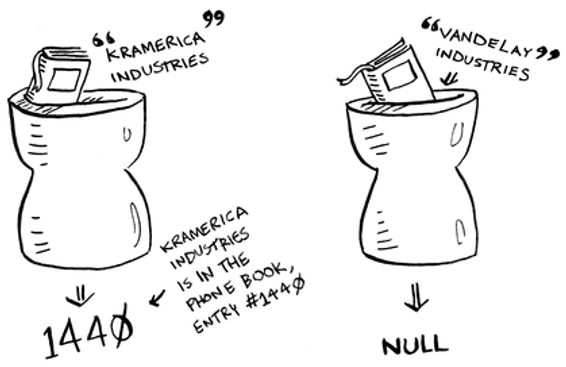
\includegraphics{./Chapter01-figure/phonebook_search.png}

\end{frame}

\begin{frame}{A Simpler Search (Problem) Example}
\protect\hypertarget{a-simpler-search-problem-example}{}

\includegraphics{./Chapter01-figure/number_search.png}

\begin{itemize}
\tightlist
\item
  I'm thinking of a number between 1 and 100.
\item
  You have to try to guess my number in the fewest tries possible.
\item
  With every guess, I'll tell you if your guess is too low, too high, or
  correct.
\end{itemize}

\end{frame}

\begin{frame}{Simple Search Way}
\protect\hypertarget{simple-search-way}{}

\begin{itemize}
\tightlist
\item
  Suppose you start guessing like this: 1, 2, 3, 4 \ldots{}.
\item
  Here's how it would go.
\end{itemize}

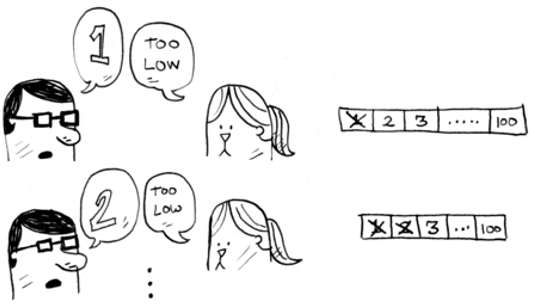
\includegraphics{./Chapter01-figure/simple_search_01.png}
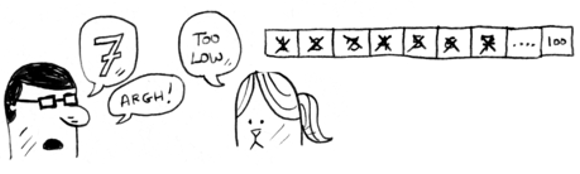
\includegraphics{./Chapter01-figure/simple_search_02.png}

\begin{itemize}
\tightlist
\item
  This is simple search (maybe stupid search would be a better term).
\item
  With each guess, you're eliminating only one number.
\item
  If my number was 99, it could take you 99 guesses to get there!
\end{itemize}

\end{frame}

\begin{frame}{A Better Way to Search (Binary Search)}
\protect\hypertarget{a-better-way-to-search-binary-search}{}

\begin{itemize}
\tightlist
\item
  Here's a better technique.
\item
  Start with 50.
\end{itemize}

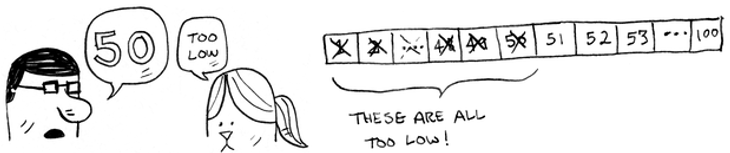
\includegraphics{./Chapter01-figure/binary_search_01.png}

\begin{itemize}
\tightlist
\item
  Too low, but you just eliminated half the numbers!
\item
  Now you know that 1--50 are all too low. Next guess: 75.
\end{itemize}

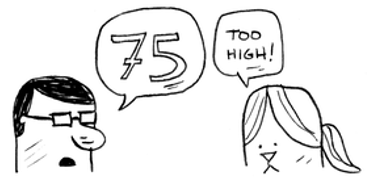
\includegraphics{./Chapter01-figure/binary_search_02.png}

\begin{itemize}
\tightlist
\item
  Too high, but again you cut down half the remaining numbers!
\item
  \textbf{With binary search, you guess the middle number and eliminate
  half the remaining numbers every time.}
\item
  Next is 63 (halfway between 50 and 75).
\end{itemize}

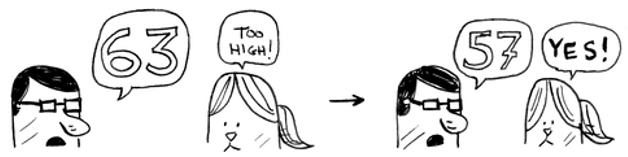
\includegraphics{./Chapter01-figure/binary_search_03.png}

\end{frame}

\begin{frame}{Binary Search Performance Explained {[}1/3{]}}
\protect\hypertarget{binary-search-performance-explained-13}{}

\begin{itemize}
\tightlist
\item
  This is binary search. You just learned your first algorithm!
\item
  Here's how many numbers you can eliminate every time.
\end{itemize}

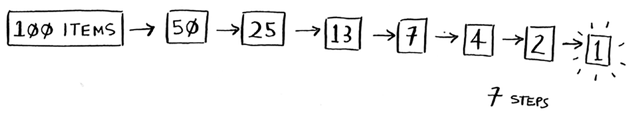
\includegraphics{./Chapter01-figure/search_steps_01.png}

\begin{itemize}
\tightlist
\item
  Eliminate half the numbers every time with binary search.
\item
  Whatever number I'm thinking of, you can guess in a maximum of seven
  guesses---because you eliminate so many numbers with every guess!
\end{itemize}

\end{frame}

\begin{frame}{Binary Search Performance Explained {[}2/3{]}}
\protect\hypertarget{binary-search-performance-explained-23}{}

\begin{itemize}
\tightlist
\item
  Suppose you're looking for a word in the dictionary. The dictionary
  has 240,000 words.
\item
  In the worst case, how many steps do you think each search will take?
\end{itemize}

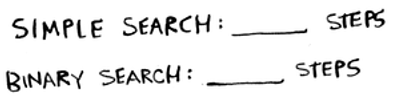
\includegraphics{./Chapter01-figure/search_steps_02.png}

\end{frame}

\begin{frame}{Binary Search Performance Explained {[}3/3{]}}
\protect\hypertarget{binary-search-performance-explained-33}{}

\begin{itemize}
\tightlist
\item
  Simple search could take 240,000 steps if the word you're looking for
  is the very last one in the book.
\item
  With each step of binary search, you cut the number of words in half
  until you're left with only one word.
\end{itemize}

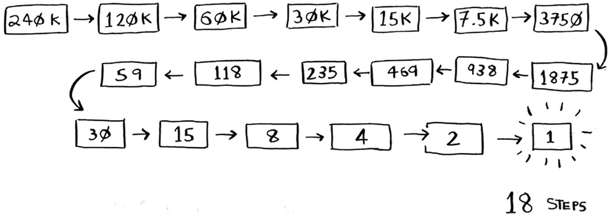
\includegraphics{./Chapter01-figure/search_steps_03.png}

\begin{itemize}
\tightlist
\item
  So binary search will take 18 steps---a big difference!
\item
  In general, for any list of \(n\), binary search will take
  \(\log_2 n\) steps to run in the worst case, whereas simple search
  will take \(n\) steps.
\end{itemize}

\end{frame}

\begin{frame}{Logarithms {[}1/2{]}}
\protect\hypertarget{logarithms-12}{}

\begin{itemize}
\tightlist
\item
  Logs are the flip of exponentials.
\end{itemize}

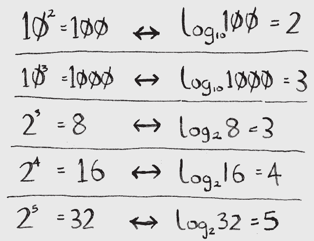
\includegraphics{./Chapter01-figure/logarithms.png}

\begin{itemize}
\tightlist
\item
  In this book, when I talk about running time in Big O notation
  (explained a little later), \(\log\) always means \(\log_2\).
\end{itemize}

\end{frame}

\begin{frame}{Logarithms {[}2/2{]}}
\protect\hypertarget{logarithms-22}{}

\begin{itemize}
\tightlist
\item
  When you search for an element using simple search, in the worst case
  you might have to look at every single element.
\item
  So for a list of 8 numbers, you'd have to check 8 numbers at most.
\item
  For binary search, you have to check \(\log n\) elements in the worst
  case.
\item
  For a list of 8 elements, \(\log 8 = 3\), because \(2^3 = 8\). So for
  a list of 8 numbers, you would have to check 3 numbers at most.
\item
  For a list of 1,024 elements, \(\log 1,024 = 10\), because
  \(2^{10} == 1,024\). So for a list of 1,024 numbers, you'd have to
  check 10 numbers at most.
\end{itemize}

\end{frame}

\begin{frame}{Notes}
\protect\hypertarget{notes}{}

\begin{itemize}
\tightlist
\item
  I'll talk about log time a lot in this book, so you should understand
  the concept of logarithms. If you don't, \textbf{Khan Academy}
  (\href{https://www.khanacademy.org/}{khanacademy.org}) has a nice
  video that makes it clear.
\item
  Binary search only works when your list is in \textbf{sorted order}.
  For example, the names in a phone book are sorted in alphabetical
  order, so you can use binary search to look for a name.
\end{itemize}

\end{frame}

\begin{frame}[fragile]{Binary Search in Python {[}1/2{]}}
\protect\hypertarget{binary-search-in-python-12}{}

\begin{itemize}
\tightlist
\item
  Let's see how to write binary search in Python.
\item
  The code sample here uses arrays.
\item
  You can store a sequence of elements in a row of consecutive buckets
  called an array.
\item
  The buckets are numbered starting with 0: the first bucket is at
  position \#0, the second is \#1, the third is \#2, and so on.
\item
  The binary\_search function takes a \textbf{sorted array} and an item.
  If the item is in the array, the function returns its position.
\item
  You'll keep track of what part of the array you have to search
  through.
\item
  At the beginning, this is the entire array:
\end{itemize}

\begin{Shaded}
\begin{Highlighting}[]
\NormalTok{low }\OperatorTok{=} \DecValTok{0}
\NormalTok{high }\OperatorTok{=} \BuiltInTok{len}\NormalTok{(}\BuiltInTok{list}\NormalTok{) }\OperatorTok{-} \DecValTok{1}
\end{Highlighting}
\end{Shaded}

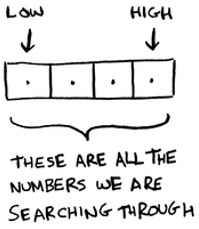
\includegraphics{./Chapter01-figure/array_binary_search_01.png}

\begin{itemize}
\tightlist
\item
  Each time, you check the middle element:
\end{itemize}

\begin{Shaded}
\begin{Highlighting}[]
\NormalTok{mid }\OperatorTok{=}\NormalTok{ (low }\OperatorTok{+}\NormalTok{ high) }\OperatorTok{/} \DecValTok{2}
\NormalTok{guess }\OperatorTok{=} \BuiltInTok{list}\NormalTok{[mid]}
\end{Highlighting}
\end{Shaded}

\begin{itemize}
\tightlist
\item
  \texttt{mid} is rounded down by Python automatically if
  \texttt{(low\ +\ high)} isn't an even number.
\item
  If the guess is too low, you update \texttt{low} accordingly:
\end{itemize}

\begin{Shaded}
\begin{Highlighting}[]
\ControlFlowTok{if}\NormalTok{ guess }\OperatorTok{<}\NormalTok{ item:}
\NormalTok{  low }\OperatorTok{=}\NormalTok{ mid }\OperatorTok{+} \DecValTok{1}
\end{Highlighting}
\end{Shaded}

\begin{itemize}
\tightlist
\item
  And if the guess is too high, you update \texttt{high}.
\end{itemize}

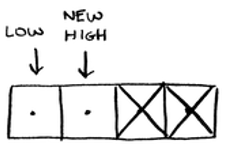
\includegraphics{./Chapter01-figure/array_binary_search_02.png}

\end{frame}

\begin{frame}[fragile]{Binary Search in Python {[}2/2{]}}
\protect\hypertarget{binary-search-in-python-22}{}

\begin{itemize}
\tightlist
\item
  The book uses \textbf{Python 2} whereas in the class we use
  \textbf{Python 3}. There are few differences in the code.
\item
  Here's the full code:
\end{itemize}

\begin{Shaded}
\begin{Highlighting}[]
\KeywordTok{def}\NormalTok{ binary_search(}\BuiltInTok{list}\NormalTok{, item):}
\NormalTok{  low }\OperatorTok{=} \DecValTok{0}
\NormalTok{  high }\OperatorTok{=} \BuiltInTok{len}\NormalTok{(}\BuiltInTok{list}\NormalTok{)}\OperatorTok{-}\DecValTok{1}
  
  \ControlFlowTok{while}\NormalTok{ low }\OperatorTok{<=}\NormalTok{ high:}
\NormalTok{    mid }\OperatorTok{=}\NormalTok{ (low }\OperatorTok{+}\NormalTok{ high) }\OperatorTok{//} \DecValTok{2}
\NormalTok{    guess }\OperatorTok{=} \BuiltInTok{list}\NormalTok{[mid]}
    \ControlFlowTok{if}\NormalTok{ guess }\OperatorTok{==}\NormalTok{ item:}
      \ControlFlowTok{return}\NormalTok{ mid}
    \ControlFlowTok{if}\NormalTok{ guess }\OperatorTok{>}\NormalTok{ item:}
\NormalTok{      high }\OperatorTok{=}\NormalTok{ mid }\OperatorTok{-} \DecValTok{1}
    \ControlFlowTok{else}\NormalTok{:}
\NormalTok{      low }\OperatorTok{=}\NormalTok{ mid }\OperatorTok{+} \DecValTok{1}
  \ControlFlowTok{return} \VariableTok{None}
  
  
\NormalTok{my_list }\OperatorTok{=}\NormalTok{ [}\DecValTok{1}\NormalTok{, }\DecValTok{3}\NormalTok{, }\DecValTok{5}\NormalTok{, }\DecValTok{7}\NormalTok{, }\DecValTok{9}\NormalTok{]}
\BuiltInTok{print}\NormalTok{(binary_search(my_list, }\DecValTok{3}\NormalTok{)) }\CommentTok{# => 1}
\end{Highlighting}
\end{Shaded}

\begin{verbatim}
## 1
\end{verbatim}

\begin{Shaded}
\begin{Highlighting}[]
\BuiltInTok{print}\NormalTok{(binary_search(my_list, }\DecValTok{-1}\NormalTok{)) }\CommentTok{# => None}
\end{Highlighting}
\end{Shaded}

\begin{verbatim}
## None
\end{verbatim}

\end{frame}

\begin{frame}{Exercises (Binary Search)}
\protect\hypertarget{exercises-binary-search}{}

Please refer to \textbf{page 9} of the textbook for exercises

\end{frame}

\begin{frame}{Running Time {[}1/2{]}}
\protect\hypertarget{running-time-12}{}

\begin{itemize}
\tightlist
\item
  Generally you want to choose the most efficient algorithm; whether
  you're trying to optimize for time or space.
\item
  Back to binary search. How much time do you save by using it?
\item
  Well, the first approach was to check each number, one by one. If this
  is a list of 100 numbers, it takes up to 100 guesses. If it's a list
  of 4 billion numbers, it takes up to 4 billion guesses.
\item
  So the maximum number of guesses is the same as the size of the list.
  This is called \textbf{linear time}.
\item
  Binary search is different. If the list is 100 items long, it takes at
  most 7 guesses. If the list is 4 billion items, it takes at most 32
  guesses.
\item
  Binary search runs in \textbf{logarithmic time} (or log time, as the
  natives call it).
\end{itemize}

\end{frame}

\begin{frame}{Running Time {[}2/2{]}}
\protect\hypertarget{running-time-22}{}

Run times for search algorithms

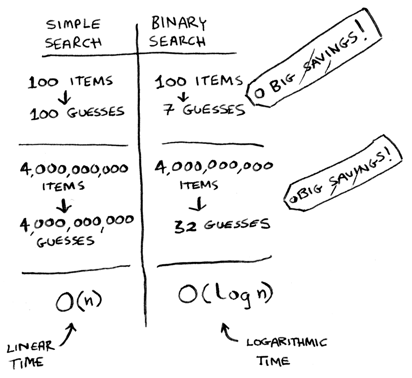
\includegraphics{./Chapter01-figure/running_time.png}

\end{frame}

\begin{frame}{Big O Notation}
\protect\hypertarget{big-o-notation}{}

\begin{itemize}
\tightlist
\item
  Big O notation is special notation that tells you how fast an
  algorithm is.
\item
  Who cares? Well, it turns out that you'll use other people's
  algorithms often---and when you do, it's nice to understand how fast
  or slow they are.
\item
  In this section, I'll explain what Big O notation is and give you a
  list of the most common running times for algorithms using it.
\end{itemize}

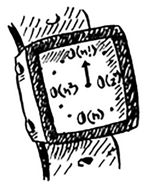
\includegraphics{./Chapter01-figure/big_o_clock.png}

\end{frame}

\begin{frame}{Algorithm running times grow at different rates {[}1/6{]}}
\protect\hypertarget{algorithm-running-times-grow-at-different-rates-16}{}

\begin{itemize}
\tightlist
\item
  Bob is writing a search algorithm for NASA.
\item
  His algorithm will kick in when a rocket is about to land on the Moon,
  and it will help calculate where to land.
\item
  And Bob has only 10 seconds to figure out where to land.
\end{itemize}

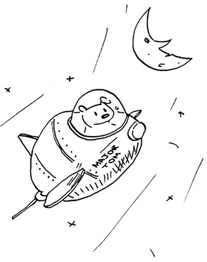
\includegraphics{./Chapter01-figure/bob_rocket.png}

\end{frame}

\begin{frame}{Algorithm running times grow at different rates {[}2/6{]}}
\protect\hypertarget{algorithm-running-times-grow-at-different-rates-26}{}

\begin{itemize}
\tightlist
\item
  Bob is trying to decide between simple search and binary search.
\item
  The algorithm needs to be both fast and correct.
\item
  On one hand, binary search is faster.
\item
  On the other hand, simple search is easier to write, and there is less
  chance of bugs being introduced. And Bob really doesn't want bugs in
  the code to land a rocket!
\end{itemize}

\end{frame}

\begin{frame}{Algorithm running times grow at different rates {[}3/6{]}}
\protect\hypertarget{algorithm-running-times-grow-at-different-rates-36}{}

\begin{itemize}
\tightlist
\item
  Let's assume it takes 1 millisecond to check one element.
\item
  To be extra careful, Bob decides to time both algorithms with a list
  of 100 elements.
\item
  With simple search, Bob has to check 100 elements, so the search takes
  100 ms to run.
\item
  On the other hand, he only has to check 7 elements with binary search
  (\(\log_2 100\) is roughly 7), so that search takes 7 ms to run.
\end{itemize}

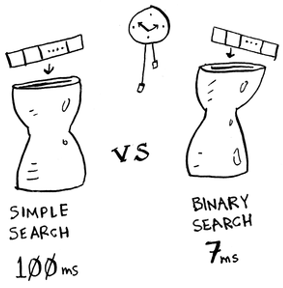
\includegraphics{./Chapter01-figure/rocket_simple_vs_binary_search.png}

\end{frame}

\begin{frame}{Algorithm running times grow at different rates {[}4/6{]}}
\protect\hypertarget{algorithm-running-times-grow-at-different-rates-46}{}

\begin{itemize}
\tightlist
\item
  But realistically, the list will have more like a billion elements.
\item
  Bob runs binary search with 1 billion elements, and it takes 30 ms
  (\(\log_2 1,000,000,000\) is roughly 30).
\item
  ``Binary search is about 15 times faster than simple search, because
  simple search took 100 ms with 100 elements, and binary search took 7
  ms.
\item
  So simple search will take 30 × 15 = 450 ms, right? Way under my
  threshold of 10 seconds.''
\item
  Bob decides to go with simple search.
\item
  \textbf{Is that the right choice?}
\end{itemize}

\end{frame}

\begin{frame}{Algorithm running times grow at different rates {[}5/6{]}}
\protect\hypertarget{algorithm-running-times-grow-at-different-rates-56}{}

\begin{itemize}
\tightlist
\item
  No.~Turns out, Bob is wrong. Dead wrong.
\item
  The run time for simple search with 1 billion items will be 1 billion
  ms, which is 11 days!
\item
  The problem is, the run times for binary search and simple search
  \textbf{don't grow at the same rate}.
\end{itemize}

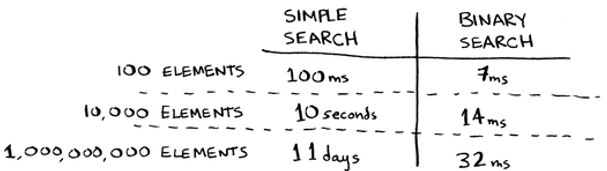
\includegraphics{./Chapter01-figure/different_growth_rate.png}

\end{frame}

\begin{frame}{Algorithm running times grow at different rates {[}6/6{]}}
\protect\hypertarget{algorithm-running-times-grow-at-different-rates-66}{}

\begin{itemize}
\item
  As the number of items increases, binary search takes a little more
  time to run. But simple search takes a lot more time to run.
\item
  So as the list of numbers gets bigger, binary search suddenly becomes
  a lot faster than simple search.
\item
  That's why it's not enough to know how long an algorithm takes to
  run---you need to know how the running time increases as the list size
  increases.
\item
  That's where Big O notation comes in.
\end{itemize}

\end{frame}

\begin{frame}{Big O Notation Explained {[}1/2{]}}
\protect\hypertarget{big-o-notation-explained-12}{}

\begin{itemize}
\tightlist
\item
  Big O notation tells you how fast an algorithm is.
\item
  For example, suppose you have a list of size \(n\).
\item
  Simple search needs to check each element, so it will take \(n\)
  operations. The run time in Big O notation is \(O(n)\).
\item
  Big O \textbf{doesn't tell you the speed in seconds}. Big O notation
  lets you compare the number of operations. It tells you \textbf{how
  fast the algorithm grows}.
\end{itemize}

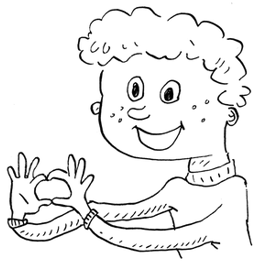
\includegraphics{./Chapter01-figure/big_o_hand_gesture.png}

\end{frame}

\begin{frame}{Big O Notation Explained {[}2/2{]}}
\protect\hypertarget{big-o-notation-explained-22}{}

\begin{itemize}
\tightlist
\item
  Binary search needs log n operations to check a list of size \(n\).
\item
  What's the running time in Big O notation? It's \(O_{(\log n)}\).
\item
  In general, Big O notation is written as follows.
\end{itemize}

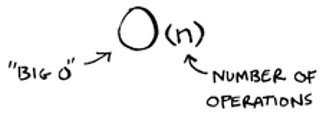
\includegraphics{./Chapter01-figure/big_o_notation.png}

\begin{itemize}
\tightlist
\item
  This tells you the number of operations an algorithm will make.
\item
  It's called Big O notation because you put a ``big O'' in front of the
  number of operations (it sounds like a joke, but it's true!).
\end{itemize}

\end{frame}

\begin{frame}{Visualizing different Big O run times (another simple case
study)}
\protect\hypertarget{visualizing-different-big-o-run-times-another-simple-case-study}{}

\begin{itemize}
\tightlist
\item
  Here's a practical example you can follow at home with a few pieces of
  paper and a pencil.
\item
  Suppose you have to draw a grid of 16 boxes.
\end{itemize}

\begin{figure}
\centering
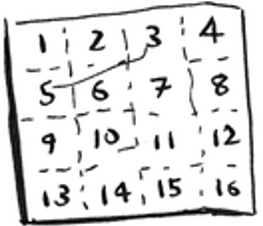
\includegraphics{./Chapter01-figure/grid_drawing_01.png}
\caption{What's a good algorithm to draw this grid?}
\end{figure}

\end{frame}

\begin{frame}{Algorithm 1}
\protect\hypertarget{algorithm-1}{}

\begin{itemize}
\tightlist
\item
  One way to do it is to draw 16 boxes, one at a time.
\item
  Remember, Big O notation counts the number of operations.
\item
  In this example, drawing one box is one operation. You have to draw 16
  boxes.
\item
  How many operations will it take, drawing one box at a time?
\end{itemize}


\includegraphics{./Chapter01-figure/grid_drawing_02.png}

\begin{itemize}
\tightlist
\item
  It takes 16 steps to draw 16 boxes. What's the running time for this
  algorithm?
\end{itemize}

\end{frame}

\begin{frame}{Algorithm 2 {[}1/3{]}}
\protect\hypertarget{algorithm-2-13}{}

\begin{itemize}
\tightlist
\item
  Try this algorithm instead. Fold the paper.
\end{itemize}


\includegraphics{./Chapter01-figure/grid_drawing_03.png}

\begin{itemize}
\tightlist
\item
  In this example, folding the paper once is an operation.
\item
  You just made two boxes with that operation!
\end{itemize}

\end{frame}

\begin{frame}{Algorithm 2 {[}2/3{]}}
\protect\hypertarget{algorithm-2-23}{}

\begin{itemize}
\tightlist
\item
  Fold the paper again, and again, and again.
\end{itemize}

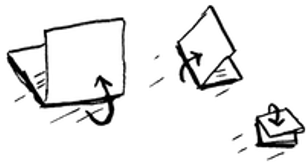
\includegraphics{./Chapter01-figure/grid_drawing_04.png}

\begin{itemize}
\tightlist
\item
  Unfold it after four folds, and you'll have a beautiful grid!
\end{itemize}

\end{frame}

\begin{frame}{Algorithm 2 {[}3/3{]}}
\protect\hypertarget{algorithm-2-33}{}

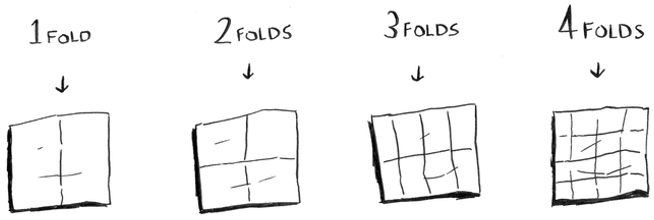
\includegraphics{./Chapter01-figure/grid_drawing_05.png}

\begin{itemize}
\tightlist
\item
  Every fold doubles the number of boxes. You made 16 boxes with 4
  operations!
\item
  You can ``draw'' twice as many boxes with every fold, so you can draw
  16 boxes in 4 steps.
\item
  What's the running time for this algorithm?
\item
  Come up with running times for both algorithms before moving on.
\item
  Answers: Algorithm 1 takes \(O(n)\) time, and algorithm 2 takes
  \(O(\log n)\) time.
\end{itemize}

\end{frame}

\begin{frame}{Big O establishes a worst-case run time {[}1/2{]}}
\protect\hypertarget{big-o-establishes-a-worst-case-run-time-12}{}

\begin{itemize}
\tightlist
\item
  Suppose you're using simple search to look for a person in the phone
  book.
\item
  You know that simple search takes \(O(n)\) time to run, which means in
  the worst case, you'll have to look through every single entry in your
  phone book.
\item
  In this case, you're looking for Adit. This guy is the first entry in
  your phone book. So you didn't have to look at every entry---you found
  it on the first try.
\item
  Did this algorithm take \(O(n)\) time? Or did it take \(O(1)\) time
  because you found the person on the first try?
\end{itemize}

\end{frame}

\begin{frame}{Big O establishes a worst-case run time {[}2/2{]}}
\protect\hypertarget{big-o-establishes-a-worst-case-run-time-22}{}

\begin{itemize}
\tightlist
\item
  Simple search still takes \(O(n)\) time.
\item
  In this case, you found what you were looking for instantly. That's
  the best-case scenario.
\item
  But \textbf{Big O notation} is about \textbf{the worst-case scenario}.
\item
  So you can say that, in the worst case, you'll have to look at every
  entry in the phone book once. That's \(O(n)\) time.
\item
  It's a reassurance---you know that simple search will never be slower
  than \(O(n)\) time.
\end{itemize}

\end{frame}

\begin{frame}{Some common Big O run times {[}1/4{]}}
\protect\hypertarget{some-common-big-o-run-times-14}{}

Here are five Big O run times that you'll encounter a lot, sorted from
fastest to slowest:

\begin{itemize}
\tightlist
\item
  \(O(\log n)\), also known as log time. Example: Binary search.
\item
  \(O(n)\), also known as linear time. Example: Simple search.
\item
  \(O(n * \log n)\). Example: A fast sorting algorithm, like quicksort
  (coming up in chapter 4).
\item
  \(O(n^2 )\). Example: A slow sorting algorithm, like selection sort
  (coming up in chapter 2).
\item
  \(O(n!)\). Example: A really slow algorithm, like the traveling sales
  person (coming up next!).
\end{itemize}

\end{frame}

\begin{frame}{Some common Big O run times {[}2/4{]}}
\protect\hypertarget{some-common-big-o-run-times-24}{}

\begin{itemize}
\tightlist
\item
  Suppose you're drawing a grid of 16 boxes again, and you can choose
  from 5 different algorithms to do so.
\item
  You can do 10 operations per second.
\item
  If you use the first algorithm, it will take you \(O(\log n)\) time to
  draw the grid.\\
\item
  With O(log n) time, it will take you 4 operations to draw a grid of 16
  boxes (log 16 is 4). So it will take you 0.4 seconds to draw the grid.
\item
  What if you have to draw 1,024 boxes? It will take you
  \(\log 1,024 = 10\) operations, or 1 second to draw a grid of 1,024
  boxes.
\item
  These numbers are using the first algorithm.
\end{itemize}

\end{frame}

\begin{frame}{Some common Big O run times {[}3/4{]}}
\protect\hypertarget{some-common-big-o-run-times-34}{}

\begin{itemize}
\tightlist
\item
  The second algorithm is slower: it takes O(n) time.
\item
  It will take 16 operations to draw 16 boxes, and it will take 1,024
  operations to draw 1,024 boxes.
\item
  How much time is that in seconds?
\end{itemize}

\end{frame}

\begin{frame}{Some common Big O run times {[}4/4{]}}
\protect\hypertarget{some-common-big-o-run-times-44}{}

\begin{itemize}
\tightlist
\item
  Here's how long it would take to draw a grid for the rest of the
  algorithms, from fastest to slowest:
\end{itemize}

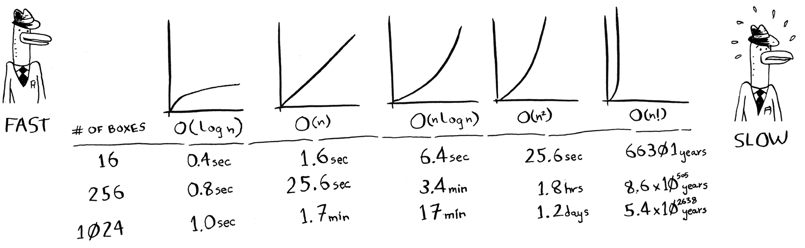
\includegraphics{./Chapter01-figure/big_o_fast_to_slow.png}

\begin{itemize}
\tightlist
\item
  There are other run times, too, but these are the five most common.
\item
  This is a simplification. In reality you can't convert from a Big O
  run time to a number of operations this neatly, but this is good
  enough for now.
\end{itemize}

\end{frame}

\begin{frame}{Big O Notation (recap)}
\protect\hypertarget{big-o-notation-recap}{}

For now, the main takeaways are as follows:

\begin{itemize}
\tightlist
\item
  Algorithm speed isn't measured in seconds, but in growth of the number
  of operations.
\item
  Instead, we talk about how quickly the run time of an algorithm
  increases as the size of the input increases.
\item
  Run time of algorithms is expressed in Big O notation.
\item
  \(O(\log n)\) is faster than \(O(n)\), but it gets a lot faster as the
  list of items you're searching grows.
\end{itemize}

\end{frame}

\begin{frame}{Exercises (Big O Notation)}
\protect\hypertarget{exercises-big-o-notation}{}

Please refer to \textbf{page 17} of the textbook for exercises

\end{frame}

\begin{frame}{The Traveling Salesperson Problem {[}1/6{]}}
\protect\hypertarget{the-traveling-salesperson-problem-16}{}

\begin{itemize}
\tightlist
\item
  You might have read that last section and thought, ``There's no way
  I'll ever run into an algorithm that takes O(n!) time.''
\item
  Well, let me try to prove you wrong!
\item
  Here's an example of an algorithm with a really bad running time.
\item
  This is a famous problem in computer science, because its growth is
  appalling and some very smart people think it can't be improved.
\item
  It's called \textbf{the traveling salesperson problem}.
\end{itemize}

\end{frame}

\begin{frame}{The Traveling Salesperson Problem {[}2/6{]}}
\protect\hypertarget{the-traveling-salesperson-problem-26}{}

You have a salesperson


\includegraphics{./Chapter01-figure/travelling_salesperson_01.png}

\end{frame}

\begin{frame}{The Traveling Salesperson Problem {[}3/6{]}}
\protect\hypertarget{the-traveling-salesperson-problem-36}{}

The salesperson has to go to five cities

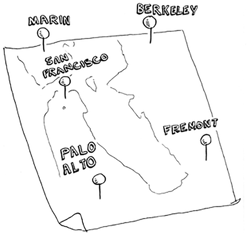
\includegraphics{./Chapter01-figure/travelling_salesperson_02.png}

\end{frame}

\begin{frame}{The Traveling Salesperson Problem {[}4/6{]}}
\protect\hypertarget{the-traveling-salesperson-problem-46}{}

\begin{itemize}
\tightlist
\item
  This salesperson, whom I'll call Opus, wants to hit all five cities
  while traveling the minimum distance.
\item
  Here's one way to do that: look at every possible order in which he
  could travel to the cities.
\end{itemize}

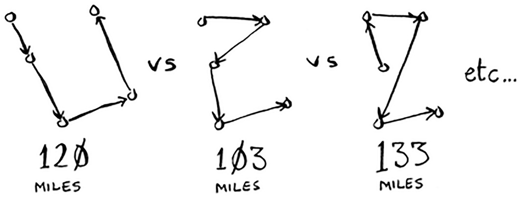
\includegraphics{./Chapter01-figure/travelling_salesperson_03.png}

\end{frame}

\begin{frame}{The Traveling Salesperson Problem {[}5/6{]}}
\protect\hypertarget{the-traveling-salesperson-problem-56}{}

\begin{itemize}
\tightlist
\item
  He adds up the total distance and then picks the path with the lowest
  distance.
\item
  There are 120 permutations with 5 cities, so it will take 120
  operations to solve the problem for 5 cities.
\item
  For 6 cities, it will take 720 operations (there are 720
  permutations).
\item
  For 7 cities, it will take 5,040 operations!
\end{itemize}

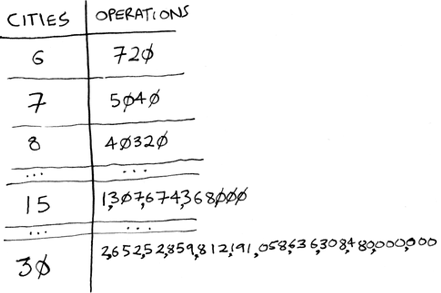
\includegraphics{./Chapter01-figure/travelling_salesperson_04.png}

\end{frame}

\begin{frame}{The Traveling Salesperson Problem {[}6/6{]}}
\protect\hypertarget{the-traveling-salesperson-problem-66}{}

\begin{itemize}
\tightlist
\item
  In general, for \(n\) items, it will take \(n!\) (\(n\) factorial)
  operations to compute the result.
\item
  So this is \(O(n!)\) time, or factorial time.
\item
  It takes a lot of operations for everything except the smallest
  numbers.
\item
  Once you're dealing with 100+ cities, it's impossible to calculate the
  answer in time.
\item
  This is a terrible algorithm! Opus should use a different one, right?
\item
  But he can't. This is one of the unsolved problems in computer
  science.
\item
  There's no fast known algorithm for it, and smart people think it's
  impossible to have a smart algorithm for this problem.
\item
  The best we can do is come up with an approximate solution.
\end{itemize}

\end{frame}

\begin{frame}{Recap}
\protect\hypertarget{recap}{}

\begin{itemize}
\tightlist
\item
  Binary search is a lot faster than simple search.
\item
  \(O(\log n)\) is faster than \(O(n)\), but it gets a lot faster once
  the list of items you're searching through grows.
\item
  Algorithm speed isn't measured in seconds.
\item
  Algorithm times are measured in terms of growth of an algorithm.
\item
  Algorithm times are written in Big O notation.
\end{itemize}

\end{frame}

\end{document}
